\section{Temporal stability}
The following section will be looking at the results from choosing different $\theta$ values in our scheme. The benchmark test FSI-2 has been used to with a pretty high time step $ k = 0.01$. We only study the effects of lift as the three other quantities shows the same behavior.   
\begin{figure}[H]
\label{fig:lift_shifted}
\caption{LiftShifted}
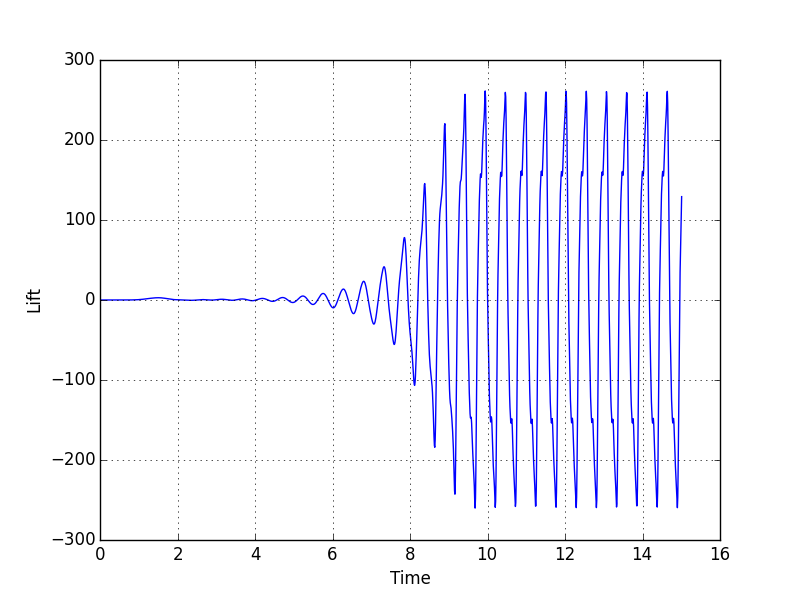
\includegraphics[scale=0.6, trim={0mm 0mm 0mm 0mm},clip]{./Verification_Validation/Temporal_stability/lift_shifted.png}
\end{figure}


\begin{figure}[H]  \label{CSM3_plots} 
  \caption {Displacement of point A, CSM3}
  \begin{minipage}[b]{0.5\linewidth}
    \centering
    \includegraphics[width=.75\linewidth]{./Verification_Validation/Temporal_stability/FSI2_001_05_big.png} 
    \caption{$ $} 
    \vspace{4ex}
  \end{minipage}%%
  \begin{minipage}[b]{0.5\linewidth}
    \centering
    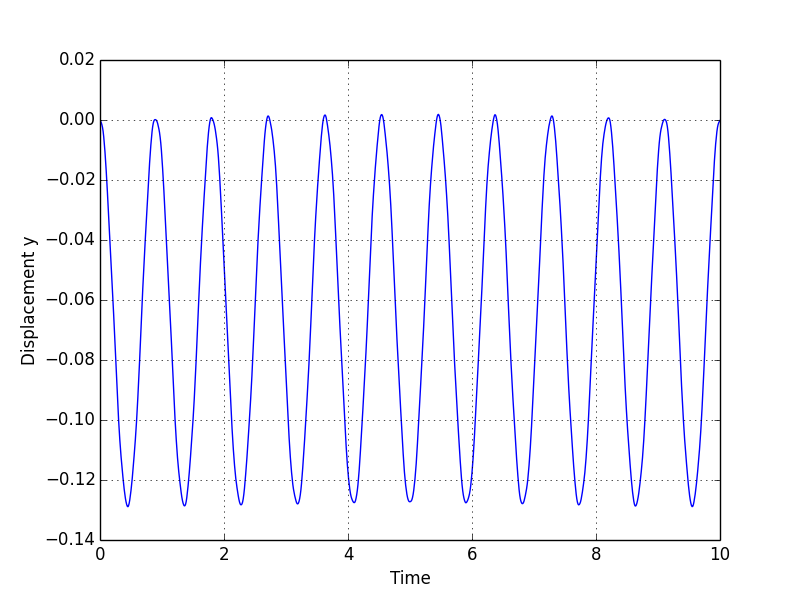
\includegraphics[width=.75\linewidth]{./Verification_Validation//Hron_Turek/dis_y.png} 
    \caption{Discplacement y} 
    \vspace{4ex}
  \end{minipage} 
  \begin{minipage}[b]{0.5\linewidth}
    \centering
    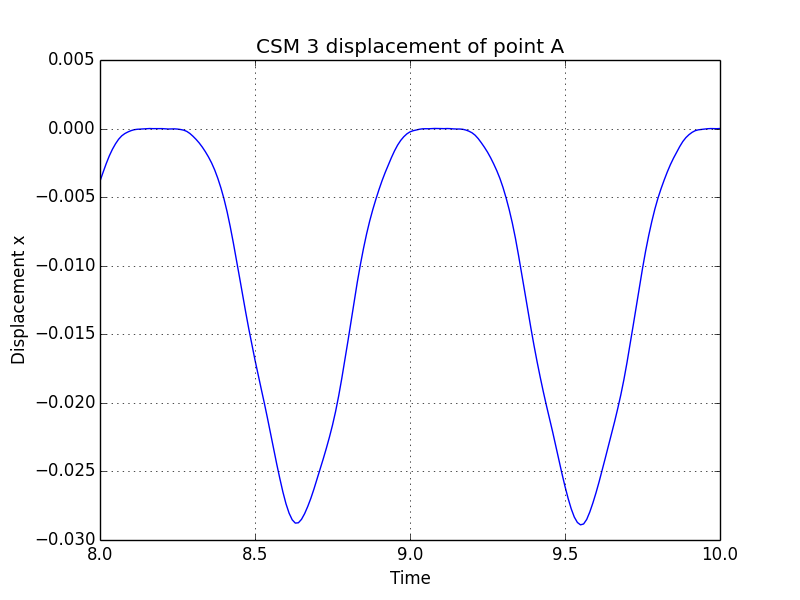
\includegraphics[width=.75\linewidth]{./Verification_Validation//Hron_Turek/dis_x_short.png} 
    \caption{Displacement x} 
    \vspace{4ex}
  \end{minipage}%% 
  \begin{minipage}[b]{0.5\linewidth}
    \centering
    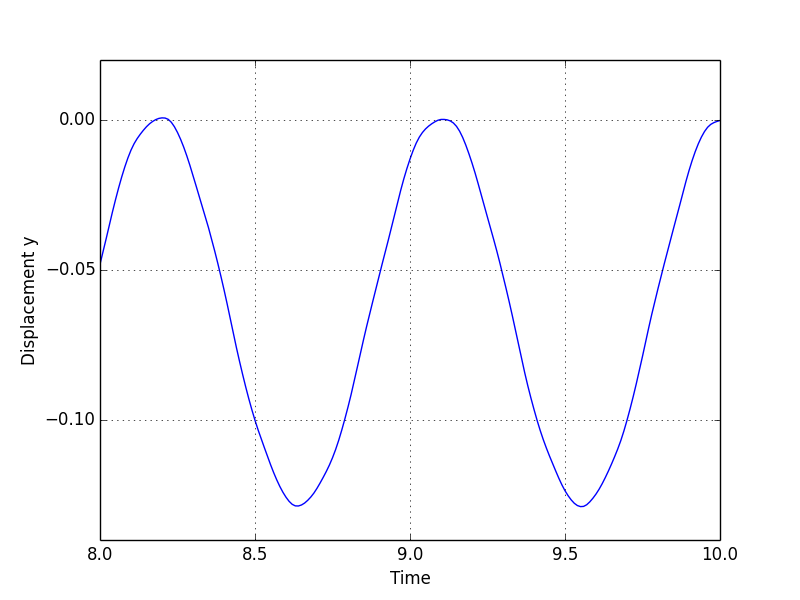
\includegraphics[width=.75\linewidth]{./Verification_Validation/Hron_Turek/dis_y_short.png} 
    \caption{Discplacement y} 
    \vspace{4ex}
  \end{minipage} 
\end{figure}
